% questions.tex —— 2016 年·山东卷·理科 · 题目内容片段（无答案）
% 由 tools/generate_projects.py 依来源总账自 2016/2016_数学真题_山东理_试题.md 生成，勿手改（改源 MD 后重跑）


\gkpart{数学}

\begin{gktip}
\textbf{来源说明}：本题面依据固定源 PDF 两页 A3 页面逐题核对，原卷印刷页码 1011–1012。固定源不附答案、不印分值；本文件仅为题面规范源。源内中文标点一律为半角，本文件按项目约定统一为全角；源内异常一律照录并在 \texttt{.work} 版式文件中逐条登记（第 1 题「\(3-2i\)」与「其中」之间源内无标点，照录；第 17 题图未按 \(AB=BC\) 精确作图，为示意）。
\end{gktip}

\gkpart{一、选择题}

\begin{question}
\gkti{1}若复数 \(z\) 满足 \(2z+\overline{z}=3-2i\) 其中 \(i\) 为虚数单位，则 \(z=\)（　）

（A）\(1+2i\)　（B）\(1-2i\)　（C）\(-1+2i\)　（D）\(-1-2i\)

\end{question}
\begin{question}
\gkti{2}设集合 \(A=\{y\mid y=2^{x},x\in\mathbf{R}\}\)，\(B=\{x\mid x^{2}-1<0\}\)，则 \(A\cup B=\)（　）

（A）\((-1,1)\)　（B）\((0,1)\)　（C）\((-1,+\infty)\)　（D）\((0,+\infty)\)

\Needspace{0.4\textheight}
\end{question}
\begin{question}
\gkti{3}某高校调查了 \(200\) 名学生每周的自习时间（单位：小时），制成了如图所示的频率分布直方图，其中自习时间的范围是 \([17.5,30]\)，样本数据分组为 \([17.5,20)\)，\([20,22.5)\)，\([22.5,25)\)，\([25,27.5)\)，\([27.5,30]\)。根据直方图，这 \(200\) 名学生中每周的自习时间不少于 \(22.5\) 小时的人数是（　）
\nopagebreak[4]
\begin{center}% 第 3 题频率分布直方图：按固定源 PDF 矢量路径实测重绘（1 pt → 0.03515 cm）。
% 原点取轴交点（源页 (132.48, 458.06) pt），y 向上。组距 2.5 小时 = 21.26 pt（横轴 1 组 = 21.26）。
% 纵轴刻度自下而上 0.02/0.04/0.08/0.10/0.16（无 0 标签，非单调步长）；柱高依次 0.02/0.10/0.16/0.08/0.04
% （实测 14.17/70.85/113.35/56.67/28.33 pt，与刻度完全自洽）。
% 5 条水平虚线自纵轴右行、止于对应柱左边缘（横穿其左侧各柱）；纵轴标签「频率／组距」为竖排分数式。
\begin{tikzpicture}[>=stealth,every node/.style={font=\small},x=0.03515cm,y=0.03515cm]
% 坐标轴（纵轴至 138.10、横轴至 166.43，箭头实心）
\draw[->] (0,0)--(0,141.7);
\draw[->] (0,0)--(170.0,0);
% 柱（高 0.02/0.10/0.16/0.08/0.04，组距 21.26）
\foreach \i/\h in {0/14.17, 1/70.85, 2/113.35, 3/56.67, 4/28.33} {
  \draw ({21.25+21.26*\i},0) rectangle ({21.25+21.26*(\i+1)},{\h});
}
% 水平虚线引导线（自纵轴至对应柱左缘）
\draw[dash pattern=on 2.99pt off 2.99pt] (0,14.17)--(21.25,14.17);
\draw[dash pattern=on 2.99pt off 2.99pt] (0,70.85)--(42.51,70.85);
\draw[dash pattern=on 2.99pt off 2.99pt] (0,113.35)--(63.77,113.35);
\draw[dash pattern=on 2.99pt off 2.99pt] (0,56.67)--(85.03,56.67);
\draw[dash pattern=on 2.99pt off 2.99pt] (0,28.33)--(106.29,28.33);
% 纵轴刻度标签（虚线高度处，纵轴左侧）
\node[left] at (-2.4,14.17) {\(0.02\)};
\node[left] at (-2.4,28.33) {\(0.04\)};
\node[left] at (-2.4,56.67) {\(0.08\)};
\node[left] at (-2.4,70.85) {\(0.10\)};
\node[left] at (-2.4,113.35) {\(0.16\)};
% 横轴刻度标签（组边界，居中于刻度）
\node[below] at (0,-2.6) {\(0\)};
\foreach \t/\x in {17.5/21.25, 20/42.51, 22.5/63.77, 25/85.03, 27.5/106.29, 30/127.55} {
  \node[below] at (\x,-2.6) {\(\t\)};
}
% 纵轴标签「频率／组距」竖排分数式（源页为分式排法：频率在上、横线、组距在下）
\node[anchor=west,inner sep=0] at (4.89,145.5) {频率};
\draw (4.89,140.99)--(25.89,140.99);
\node[anchor=west,inner sep=0] at (4.89,131.2) {组距};
% 横轴标签「自习时间/小时」（横轴上方、右端；基线在横轴上方 6.32）
\node[anchor=base west,inner sep=0] at (135.9,6.32) {自习时间/小时};
\end{tikzpicture}
\end{center}
\nopagebreak[4]
（A）\(56\)　（B）\(60\)　（C）\(120\)　（D）\(140\)

\end{question}
\begin{question}
\gkti{4}若变量 \(x,y\) 满足

\nopagebreak[4]
\[
\begin{cases}
x+y\leqslant 2,\\
2x-3y\leqslant 9,\\
x\geqslant 0,
\end{cases}
\]

则 \(x^{2}+y^{2}\) 的最大值是（　）

（A）\(4\)　（B）\(9\)　（C）\(10\)　（D）\(12\)

\Needspace{0.4\textheight}
\end{question}
\begin{question}
\gkti{5}一个由半球和四棱锥组成的几何体，其三视图如图所示。则该几何体的体积为（　）
\nopagebreak[4]
\begin{center}% 第 5 题三视图（半球＋四棱锥）：按固定源 PDF 矢量路径换算（1 pt → 0.03515 cm）。
% 原点取图组左下（源页 (156.82, 781.34) pt），y 向上。1 单位 = 34.00 pt：三角形底=高=34.00（1 单位）。
% 正（主）视图＝上半圆（r 24.05＝√2/2 单位，圆心的平边落在三角形顶点上，半圆不画平边弦）
% ＋等腰三角形；侧（左）视图与之全等（右移 85.01）；俯视图＝实线圆（r 24.05）＋虚线内接正方形
% （边 34.00）及其两条对角线。尺寸「1」共 3 处（正视图纵、横与侧视图横），俯视图无标注。
% 图注照录源内写法：「正（主）视图」「侧（左）视图」（带括注）、「俯视图」（无括注）。
\begin{tikzpicture}[>=stealth,every node/.style={font=\small},x=0.03515cm,y=0.03515cm]
% ===== 正（主）视图 =====
\draw (48.09,137.39) arc[start angle=0,end angle=180,radius=24.05];
\draw (24.04,137.39)--(7.04,103.39)--(41.04,103.39)--cycle;
% 纵向尺寸线（x=1.94，两段让位给标注；端部实心箭头；界外延长线两条）
\draw[->] (1.94,127.19)--(1.94,137.39);
\draw[->] (1.94,113.59)--(1.94,103.39);
\node at (2.0,119.5) {\(1\)};
\draw (-1.46,137.39)--(24.04,137.39);
\draw (-1.46,103.39)--(5.34,103.39);
% 横向尺寸线（y=98.29，两段让位；端部箭头；竖直端线两条）
\draw[->] (18.94,98.29)--(7.04,98.29);
\draw[->] (29.14,98.29)--(41.04,98.29);
\node at (24.12,98.29) {\(1\)};
\draw (7.04,94.89)--(7.04,101.69);
\draw (41.04,94.89)--(41.04,101.69);
% ===== 侧（左）视图（与正视图全等，右移 85.01）=====
\draw (133.10,137.39) arc[start angle=0,end angle=180,radius=24.05];
\draw (109.05,137.39)--(92.05,103.39)--(126.05,103.39)--cycle;
\draw[->] (103.95,98.29)--(92.05,98.29);
\draw[->] (114.15,98.29)--(126.05,98.29);
\node at (109.13,98.29) {\(1\)};
\draw (92.05,94.89)--(92.05,101.69);
\draw (126.05,94.89)--(126.05,101.69);
% ===== 俯视图 =====
\draw (24.04,38.78) circle (24.05);
\draw[dash pattern=on 2.99pt off 2.99pt] (7.04,55.79)--(41.04,55.79)--(41.04,21.78)--(7.04,21.78)--cycle;
\draw[dash pattern=on 2.99pt off 2.99pt] (7.04,21.78)--(41.04,55.79);
\draw[dash pattern=on 2.99pt off 2.99pt] (41.04,21.78)--(7.04,55.79);
% ===== 图注（居中于各子图下方）=====
\node[anchor=base,inner sep=0] at (24.11,73.68) {正（主）视图};
\node[anchor=base,inner sep=0] at (109.15,73.65) {侧（左）视图};
\node[anchor=base,inner sep=0] at (24.11,0) {俯视图};
\end{tikzpicture}
\end{center}
\nopagebreak[4]
（A）\(\dfrac{1}{3}+\dfrac{2}{3}\pi\)　（B）\(\dfrac{1}{3}+\dfrac{\sqrt{2}}{3}\pi\)　（C）\(\dfrac{1}{3}+\dfrac{\sqrt{2}}{6}\pi\)　（D）\(1+\dfrac{\sqrt{2}}{6}\pi\)

\end{question}
\begin{question}
\gkti{6}已知直线 \(a,b\) 分别在两个不同的平面 \(\alpha,\beta\) 内。则“直线 \(a\) 和直线 \(b\) 相交”是“平面 \(\alpha\) 和平面 \(\beta\) 相交”的（　）

（A）充分不必要条件　（B）必要不充分条件

（C）充要条件　（D）既不充分也不必要条件

\end{question}
\begin{question}
\gkti{7}函数 \(f(x)=(\sqrt{3}\sin x+\cos x)(\sqrt{3}\cos x-\sin x)\) 的最小正周期是（　）

（A）\(\dfrac{\pi}{2}\)　（B）\(\pi\)　（C）\(\dfrac{3\pi}{2}\)　（D）\(2\pi\)

\end{question}
\begin{question}
\gkti{8}已知非零向量 \(\mathbf{m},\mathbf{n}\) 满足 \(4|\mathbf{m}|=3|\mathbf{n}|\)，\(\cos\langle\mathbf{m},\mathbf{n}\rangle=\dfrac{1}{3}\)。若 \(\mathbf{n}\perp(t\mathbf{m}+\mathbf{n})\)，则实数 \(t\) 的值为（　）

（A）\(4\)　（B）\(-4\)　（C）\(\dfrac{9}{4}\)　（D）\(-\dfrac{9}{4}\)

\end{question}
\begin{question}
\gkti{9}已知函数 \(f(x)\) 的定义域为 \(\mathbf{R}\)。当 \(x<0\) 时，\(f(x)=x^{3}-1\)；当 \(-1\leqslant x\leqslant 1\) 时，\(f(-x)=-f(x)\)；当 \(x>\dfrac{1}{2}\) 时，\(f\left(x+\dfrac{1}{2}\right)=f\left(x-\dfrac{1}{2}\right)\)。则 \(f(6)=\)（　）

（A）\(-2\)　（B）\(-1\)　（C）\(0\)　（D）\(2\)

\end{question}
\begin{question}
\gkti{10}若函数 \(y=f(x)\) 的图象上存在两点，使得函数的图象在这两点处的切线互相垂直，则称 \(y=f(x)\) 具有 \(T\) 性质。下列函数中具有 \(T\) 性质的是（　）

（A）\(y=\sin x\)　（B）\(y=\ln x\)　（C）\(y=\mathrm{e}^{x}\)　（D）\(y=x^{3}\)

\end{question}
\gkpart{二、填空题}

\Needspace{0.4\textheight}
\begin{question}
\gkti{11}执行如图的程序框图，若输入的 \(a,b\) 的值分别为 \(0\) 和 \(9\)，则输出的 \(i\) 的值为 \(\underline{\qquad}\)。
\nopagebreak[4]
\begin{center}% 第 11 题程序框图（含「输入」框——本项目首例）：按固定源 PDF 矢量路径逐框重绘（1 pt → 0.03515 cm）。
% 原点取主干竖线（源页 x 564.62）与「结束」底边（y 688.94），y 向上。共 8 框 8 箭头，全实线。
% 结构要点（易错）：「输入 a,b」与「输出 i」同为向右倾平行四边形；i=i+1 与 a=a+i,b=b-i 同高并列于右侧；
% 「否」支自菱形右顶点水平右行、折向上入 i=i+1 底边；i=i+1 的出口在其【上边】，向上至 y=118.60 后
% 折左汇入主干——汇入点在 i=1 与 a=a+i,b=b-i 之间，故循环体含处理框整段（非尾循环）。
% 判断框内为单线大于号（ASCII >），非斜线双划。
\begin{tikzpicture}[>=stealth,every node/.style={font=\small},x=0.03515cm,y=0.03515cm]
% ===== 框 =====
\draw[rounded corners=3.98pt] (-13.99,186.03) rectangle (13.99,202.87);   % 开始
\draw (-30.20,154.37)--(23.97,154.37)--(30.19,171.46)--(-23.98,171.46)--cycle; % 输入（右倾平行四边形）
\draw (-14.93,125.89) rectangle (14.93,139.80);   % i=1
\draw (-47.20,95.01) rectangle (47.20,111.32);    % a=a+i,b=b-i
\draw (61.76,95.76) rectangle (108.06,110.56);    % i=i+1（右侧同高）
\draw (0,80.36)--(34.81,71.72)--(0,63.08)--(-34.81,71.72)--cycle; % 菱形 a>b
\draw (-23.69,31.57)--(17.54,31.57)--(23.68,48.43)--(-17.55,48.43)--cycle; % 输出（右倾平行四边形）
\draw[rounded corners=3.98pt] (-13.99,0) rectangle (13.99,17.01);          % 结束
% ===== 框内文字 =====
\node at (0,194.45) {开始};
\node at (0,162.92) {输入 \(a,b\)};
\node at (0,132.85) {\(i=1\)};
\node at (0,103.17) {\(a=a+i,b=b-i\)};
\node at (84.91,103.16) {\(i=i+1\)};
\node at (0,71.72) {\(a>b\)};
\node at (0,40.00) {输出 \(i\)};
\node at (0,8.51) {结束};
% ===== 箭头（主干六段 + 否支 + 回接）=====
\draw[->] (0,185.83)--(0,171.46);   % 开始→输入
\draw[->] (0,154.37)--(0,139.80);   % 输入→i=1
\draw[->] (0,125.89)--(0,111.32);   % i=1→处理框
\draw[->] (0,95.01)--(0,80.36);     % 处理框→菱形
\draw[->] (0,63.08)--(0,48.43);     % 菱形→输出（是分支）
\draw[->] (0,31.57)--(0,17.01);     % 输出→结束
\draw[->] (34.81,71.72)--(84.91,71.72)--(84.91,95.76);  % 否支：右顶点→右→上入 i=i+1 底边
\draw[->] (84.91,110.56)--(84.91,118.60)--(0,118.60);   % 回接：i=i+1 上边→上→左汇入主干
% ===== 分支标注 =====
\node at (9.13,56.29) {是};
\node at (35.32,63.87) {否};
\end{tikzpicture}
\end{center}
\nopagebreak[4]
\end{question}
\begin{question}
\gkti{12}若 \(\left(ax^{2}+\dfrac{1}{\sqrt{x}}\right)^{5}\) 的展开式中 \(x^{5}\) 的系数是 \(-80\)，则实数 \(a=\) \(\underline{\qquad}\)。

\end{question}
\begin{question}
\gkti{13}已知双曲线 \(E:\dfrac{x^{2}}{a^{2}}-\dfrac{y^{2}}{b^{2}}=1\)（\(a>0\)，\(b>0\)），若矩形 \(ABCD\) 的四个顶点在 \(E\) 上，\(AB,CD\) 的中点为 \(E\) 的两个焦点，且 \(2|AB|=3|BC|\)，则 \(E\) 的离心率是 \(\underline{\qquad}\)。

\end{question}
\begin{question}
\gkti{14}在 \([-1,1]\) 上随机地取一个数 \(k\)，则事件“直线 \(y=kx\) 与圆 \((x-5)^{2}+y^{2}=9\) 相交”发生的概率为 \(\underline{\qquad}\)。

\end{question}
\begin{question}
\gkti{15}已知函数

\nopagebreak[4]
\[
f(x)=\begin{cases}|x|, & x\leqslant m,\\x^{2}-2mx+4m, & x>m,\end{cases}
\]

其中 \(m>0\)，若存在实数 \(b\)，使得关于 \(x\) 的方程 \(f(x)=b\) 有三个不同的根，则 \(m\) 的取值范围是 \(\underline{\qquad}\)。

\end{question}
\gkpart{三、解答题}

\begin{question}
\gkti{16}在 \(\triangle ABC\) 中，角 \(A,B,C\) 的对边分别为 \(a,b,c\)，已知 \(2(\tan A+\tan B)=\dfrac{\tan A}{\cos B}+\dfrac{\tan B}{\cos A}\)。

（1） 证明：\(a+b=2c\)；

（2） 求 \(\cos C\) 的最小值。

\Needspace{0.4\textheight}
\end{question}
\begin{question}
\gkti{17}在如图所示的圆台中，\(AC\) 是下底面圆 \(O\) 的直径，\(EF\) 是上底面圆 \(O'\) 的直径，\(FB\) 是圆台的一条母线。

（1） 已知 \(G,H\) 分别为 \(EC,FB\) 的中点，求证：\(GH\parallel\) 平面 \(ABC\)；

（2） 已知 \(EF=FB=\dfrac{1}{2}AC=2\sqrt{3}\)，\(AB=BC\)。求二面角 \(F-BC-A\) 的余弦值。
\nopagebreak[4]
\begin{center}% 第 17 题圆台图：按固定源 PDF 矢量路径换算（1 pt → 0.03515 cm）。
% 原点取图组左下（源页 (962.09, 656.43) pt），y 向上。轴竖直（上下底椭圆圆心同 x=85.40）。
% 上底整椭圆实线（r 42.70/8.22）；下底：前半（近侧）下半弧实线、后半（远侧）上半弧虚线（r 85.40/16.45）；
% 左母线＝左侧轮廓，右母线 FB。虚线 7 条：AC（过 O 的直径）、OB、AB、BC、CE、CF、GH（G、H 为 EC、FB 中点）。
% 两圆心各画实心圆点；字母位置按源字形外接框中心定位（显式坐标）。
% 注：源图未按题设 AB=BC 精确作图（矢量实测 |AB|:|BC|≈1.45:1），照源描摹，不得据图反推题设。
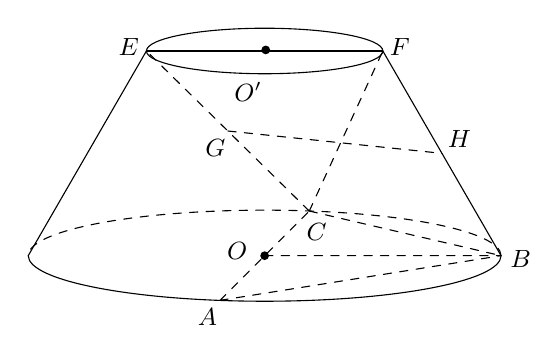
\begin{tikzpicture}[line cap=round,line join=round,font=\small,x=0.03515cm,y=0.03515cm]
% ===== 虚线先画 =====
\draw[dash pattern=on 2.99pt off 2.99pt]
  (69.26,10.70)--(101.53,42.97)   % AC（直径，过 O）
  (85.40,26.84)--(170.80,26.84)   % OB
  (69.26,10.70)--(170.80,26.84)   % AB
  (101.53,42.97)--(170.80,26.84)  % BC
  (101.53,42.97)--(42.70,100.79)  % CE（母线）
  (101.53,42.97)--(128.10,100.79) % CF（母线）
  (72.12,71.88)--(149.45,63.81);  % GH（EC、FB 中点连线）
% 下底后半（远侧）上半弧
\draw[dash pattern=on 2.99pt off 2.99pt] (170.80,26.84) arc[start angle=0,end angle=180,x radius=85.40,y radius=16.45];
% ===== 实线 =====
% 上底整椭圆
\draw (85.40,100.79) ellipse (42.70 and 8.22);
% 上底直径 EF
\draw (42.70,100.79)--(128.10,100.79);
% 两条母线（左轮廓、右母线 FB）
\draw (0,26.84)--(42.70,100.79);
\draw (128.10,100.79)--(170.80,26.84);
% 下底前半（近侧）下半弧
\draw (0,26.84) arc[start angle=180,end angle=360,x radius=85.40,y radius=16.45];
% ===== 圆心圆点 =====
\fill (85.80,101.17) circle (1.58);
\fill (85.40,26.84) circle (1.58);
% ===== 标注（显式坐标，照源字形框中心）=====
\node[anchor=center,inner sep=0] at (36.34,102.39) {$E$};
\node[anchor=center,inner sep=0] at (134.23,102.39) {$F$};
% O′ 下移至椭圆下弧之下（源位与弧相切，400 dpi 连通域实证并入；照清晰度优先原则微调）
\node[anchor=center,inner sep=0] at (79.5,86.0) {$O'$};
\node[anchor=center,inner sep=0] at (67.58,65.87) {$G$};
\node[anchor=center,inner sep=0] at (155.78,69.07) {$H$};
\node[anchor=center,inner sep=0] at (64.72,4.66) {$A$};
\node[anchor=center,inner sep=0] at (104.23,35.44) {$C$};
\node[anchor=center,inner sep=0] at (177.94,25.74) {$B$};
% O 左下移（源位紧贴圆心点与 AC 线，同上微调）
\node[anchor=center,inner sep=0] at (75.5,28.5) {$O$};
\end{tikzpicture}
\end{center}
\nopagebreak[4]
\end{question}
\begin{question}
\gkti{18}已知数列 \(\{a_{n}\}\) 的前 \(n\) 项和 \(S_{n}=3n^{2}+8n\)，\(\{b_{n}\}\) 是等差数列，且 \(a_{n}=b_{n}+b_{n+1}\)。

（1） 求数列 \(\{b_{n}\}\) 的通项公式；

（2） 令 \(c_{n}=\dfrac{(a_{n}+1)^{n+1}}{(b_{n}+2)^{n}}\)，求数列 \(\{c_{n}\}\) 的前 \(n\) 项和 \(T_{n}\)。

\end{question}
\begin{question}
\gkti{19}甲、乙两人组成“星队”参加猜成语活动，每轮活动由甲、乙各猜一个成语，在一轮活动中，如果两人都猜对，则“星队”得 \(3\) 分；如果只有一个人猜对，则“星队”得 \(1\) 分；如果两人都没猜对，则“星队”得 \(0\) 分。已知甲每轮猜对的概率是 \(\dfrac{3}{4}\)，乙每轮猜对的概率是 \(\dfrac{2}{3}\)；每轮活动中甲、乙猜对与否互不影响。各轮结果亦互不影响。假设“星队”参加两轮活动，求：

（1） “星队”至少猜对 \(3\) 个成语的概率；

（2） “星队”两轮得分之和为 \(X\) 的分布列和数学期望 \(EX\)。

\end{question}
\begin{question}
\gkti{20}已知 \(f(x)=a(x-\ln x)+\dfrac{2x-1}{x^{2}}\)，\(a\in\mathbf{R}\)。

（1） 讨论 \(f(x)\) 的单调性；

（2） 当 \(a=1\) 时，证明 \(f(x)>f'(x)+\dfrac{3}{2}\) 对于任意的 \(x\in[1,2]\) 成立。

\Needspace{0.4\textheight}
\end{question}
\begin{question}
\gkti{21}平面直角坐标系 \(xOy\) 中，椭圆 \(C:\dfrac{x^{2}}{a^{2}}+\dfrac{y^{2}}{b^{2}}=1\)（\(a>b>0\)）的离心率是 \(\dfrac{\sqrt{3}}{2}\)，抛物线 \(E:x^{2}=2y\) 的焦点 \(F\) 是 \(C\) 的一个顶点。

（1） 求椭圆 \(C\) 的方程；

（2） 设 \(P\) 是 \(E\) 上的动点，且位于第一象限，\(E\) 在点 \(P\) 处的切线 \(l\) 与 \(C\) 交于不同的两点 \(A,B\)，线段 \(AB\) 的中点为 \(D\)，直线 \(OD\) 与过 \(P\) 且垂直于 \(x\) 轴的直线交于点 \(M\)。

　　① 求证：点 \(M\) 在定直线上；

　　② 直线 \(l\) 与 \(y\) 轴交于点 \(G\)，记 \(\triangle PFG\) 的面积为 \(S_{1}\)，\(\triangle PDM\) 的面积为 \(S_{2}\)，求 \(\dfrac{S_{1}}{S_{2}}\) 的最大值及取得最大值时点 \(P\) 的坐标。
\nopagebreak[4]
\begin{center}% 第 21 题坐标图：按固定源 PDF 矢量路径换算（1 数学单位 = 85.0 pt → 2.988 cm；按比例作图）。
% 坐标原点即两轴交点；椭圆 C: x²+4y²=1（半轴 1.0/0.5，线宽 0.8）；抛物线 E: x²=2y 顶点在原点、
% 只画 x 轴以上部分（至 x=±1.2）；切线 l（斜率 0.5399）、线段 OM、过 P 的竖直线（上下均越出图形本体）、
% 线段 FP。图上无实心圆点、坐标轴无刻度。l 为斜置斜体字母。标注按源字形框中心定位（显式坐标）。
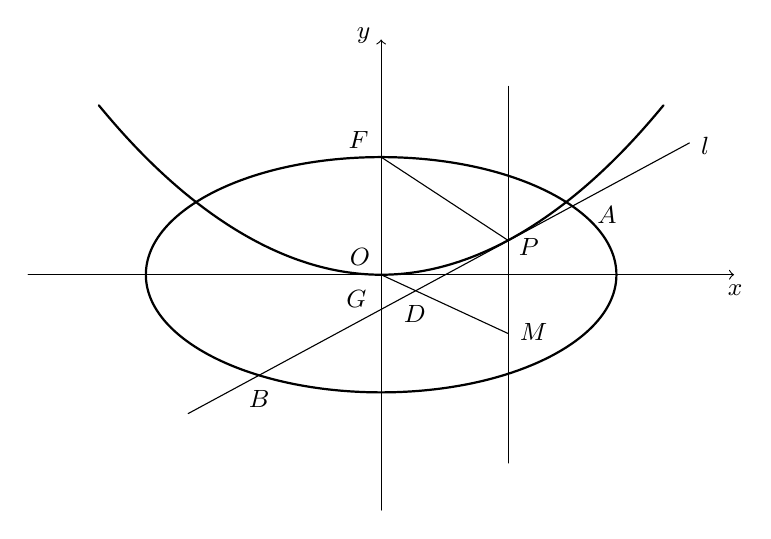
\begin{tikzpicture}[line cap=round,line join=round,font=\small,x=2.988cm,y=2.988cm]
% 坐标轴
\draw[->] (-1.50,0)--(1.50,0);
\draw[->] (0,-1.00)--(0,1.00);
% 椭圆（线宽 0.8，与源一致）与抛物线
\draw[line width=0.8pt] (0,0) ellipse (1.0 and 0.5);
\draw[line width=0.8pt] (-1.2,0.72) parabola bend (0,0) (1.2,0.72);
% 切线 l、线段 OM、过 P 的竖直线、线段 FP
\draw (-0.820,-0.590)--(1.310,0.560);
\draw (0,0)--(0.5399,-0.25);
\draw (0.5399,-0.80)--(0.5399,0.80);
\draw (0,0.5)--(0.5399,0.1458);
% ===== 标注（显式坐标，照源字形框中心）=====
\node[anchor=center,inner sep=0] at (-0.074,1.017) {\(y\)};
\node[anchor=center,inner sep=0] at (1.505,-0.066) {\(x\)};
\node[anchor=center,inner sep=0] at (-0.096,0.574) {\(F\)};
\node[anchor=center,inner sep=0] at (-0.0895,0.0741) {\(O\)};
% G 左上移（源位贴近切线，400 dpi 连通域实证并入；照清晰度优先原则微调）
\node[anchor=center,inner sep=0] at (-0.105,-0.105) {\(G\)};
\node[anchor=center,inner sep=0] at (0.6278,0.1184) {\(P\)};
\node[anchor=center,inner sep=0] at (0.6483,-0.2417) {\(M\)};
% A 右下移（源位贴近切线与椭圆，400 dpi 连通域实证并入；照清晰度优先原则微调至椭圆外）
\node[anchor=center,inner sep=0] at (0.96,0.252) {\(A\)};
\node[anchor=center,inner sep=0] at (0.143,-0.1675) {\(D\)};
\node[anchor=center,inner sep=0] at (-0.518,-0.5275) {\(B\)};
\node[anchor=center,inner sep=0] at (1.377,0.548) {\(l\)};
\end{tikzpicture}
\end{center}
\nopagebreak[4]

\end{question}